\chapter{Background}

\section{Random Access and its Limitations}\label{B:RA}
The necessity of the expansion of the existing standards of wireless networks for the effective handling of large numbers of Machine Type Communications (MTC) had already been identified by the 3GPP early in the implementation of Long Term Evolution (LTE) as a standard in \cite{3rdGenerationPartnershipProject;2011}. As explained in \cite{Laya2014}, a large amount of problems arise with increasingly large amounts of devices connecting to the Base Station (BS) or Evolved Node B (eNodeB) mostly due to the Random Access (RA) procedure that has to be initiated with every connection.

\begin{figure}[!h]
\centering
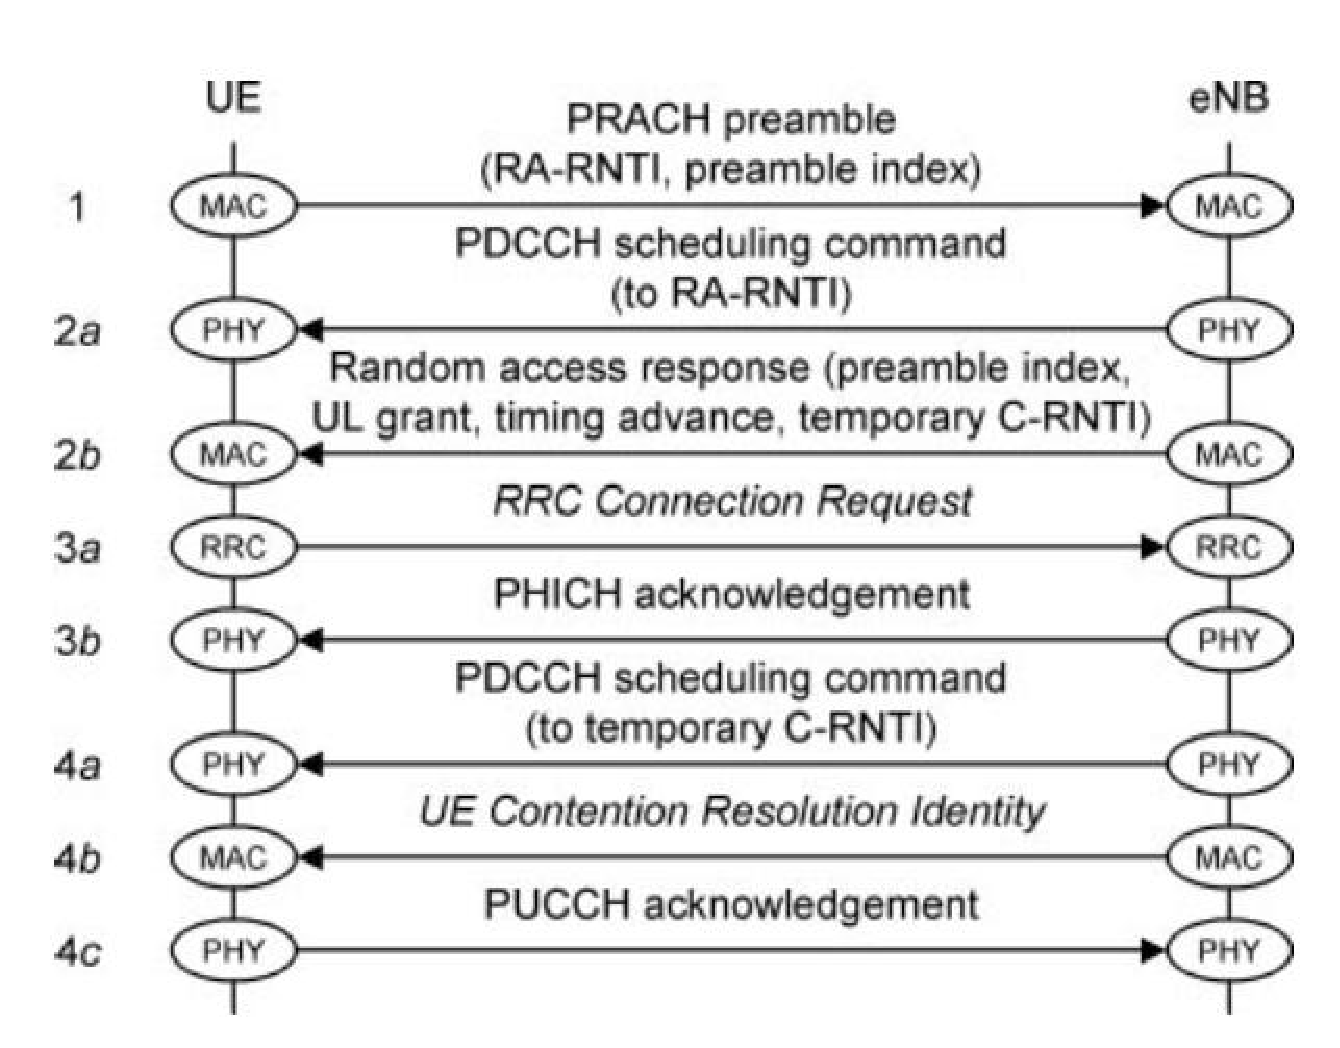
\includegraphics[scale = 0.45]{figures/Random_Access_Procedure}
\caption{Detail of the Random Access Procedure, \cite{Cox2012}}
\end{figure}

RA procedures occurr when a device intends to utilize resources on the Physical Uplink Shared Channel (PUSCH), but has not been given access to the Physical Uplink Control Channel (PUCCH) by the appropriate eNB, which is needed for a scheduling request. As described in \cite{Cox2012}, the User Equipment (UE) then sends a random access preamble to trigger the procedure, in order to gain the desired access.

This preamble is chosen randomly from an available set generated with a Zadoff-Chu mathematical sequence and transmitted on the Physical Random Access Channel (PRACH). The eNB then solves any possible collisions that may occurr from devices transmitting with the same preamble, granting access to some while ordering others to back off for a certain amount of time. If no access grant is given after several tries, the transmission is considered to have failed.

When a large amount of these connections are initiated in a short time frame, the contention resolution procedures cannot deal with them in a timely manner and many of them are dropped or delayed significantly, waiting for an opportunity to synchronize with the eNodeB, as shown in \cite{Polese2016}. This scenario occurs most often either because the transmission times are highly correlated or just due to the large number of devices in a given area. Both of these circumstances, both in isolation and in conjunction, will be very ordinary occurences in Internet of Things (IoT) and Smart City applications. 

\section{D2D}\label{B:D2D}

\section{Clustering}\label{B:Cl}
%llegar a como decidimos usar d2d en un ambiente de ciudad para probar nuestras mierdis

Many approaches have been suggested for the improvement of the circumstances described in the preceding section, as summarized succintly in \cite{Laya2014}, mostly dealing with the improvement of the RA procedures or an expansion of the standards for the Random Access Channel (RACH). Another viable alternative, as presented in a variety of papers (\cite{Wei2012a},\cite{Laya2014a},\cite{Wang2013},\cite{Liao2013}) is the clustering of transmitting devices. This approach aims to reutilize the coding and frequency resources within a given set of UEs for different ends, such as decreasing the load on the eNB, increasing the coverage area of the network or minimizing the power consumption of the units involved.

Clustering works by designating devices, called Cluster Heads (CH) that act as relays between the different UEs in a certain area and the eNB or a further Cluster Head by aggregating the data sent to it and relaying it. This aggregation can occur simply by gathering the data over a period of time and transmitting the same information in one long message, as in \cite{Shariatmadari2015}, or through actual elimination of data redundancy, as contemplated in \cite{Riker2015}.

The Cluster Heads themselves are often dedicated gateways, as utilized in \cite{Niyato2011} or \cite{Shariatmadari2015} and have been utilized especially in Wireless Sensor Networks with some frequency. Another, very promising approach to creating clusters is the use of direct Device-to-Device (D2D) communication to eliminate the need for dedicated Cluster Heads and enable dynamic cluster forming depending on the circumstances experienced by the network.

\begin{figure}[!h]
\centering
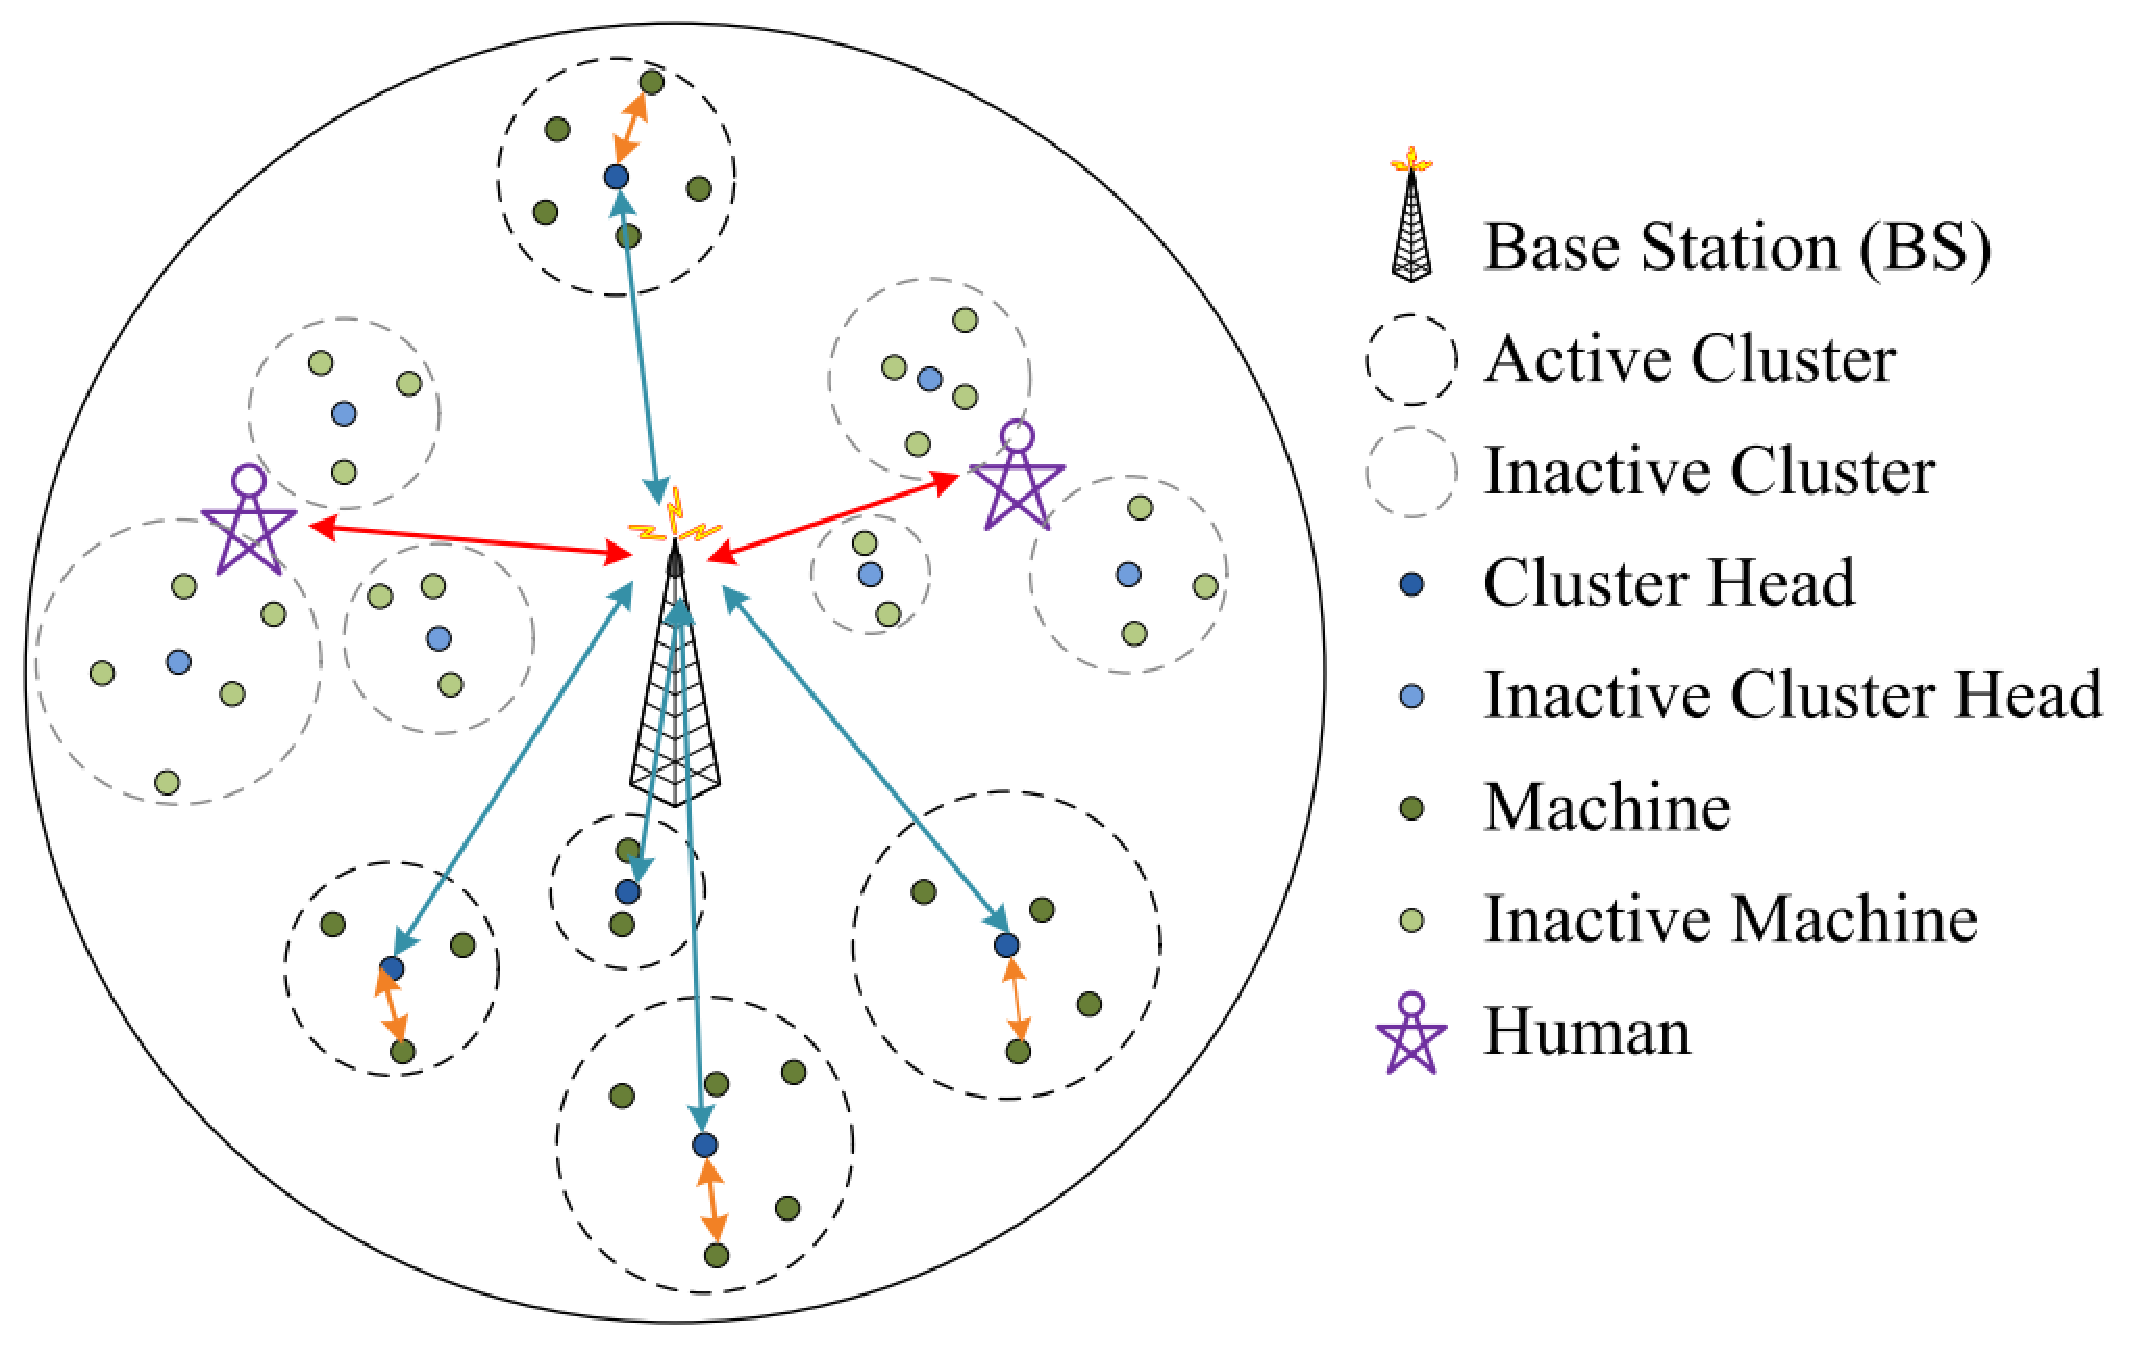
\includegraphics[scale = 0.25]{figures/D2D_clustering}
\caption{Example of D2D Clustering in a network \cite{Wang2013}}
\end{figure}

This type of clustering scheme promises to bring much needed flexibility to the creation of these structures, since they do not necessitate much investment in additional infrastructure, nor much prior information about the density of devices. D2D communications bring many benefits, both for the user and the network, but also raise several issues that have not been yet properly investigated so far, see \cite{Klugel2014}. As devices utilize the same shared resources in a constrained space, interference becomes more of an issue as devices elect to transmit their messages in the same bandwith. This topic of inter-cluster interference due to reuse of resources and its effects on possible D2D connections is of great interest to this thesis. 

As mentioned earlier, this sort of application is specially intriguing in the case of highly dense Smart Cities and the IoT. Despite the promising vistas offered by this technology, there is a dearth of research concerning this specific scenario, be it a comparison of different clustering schemes or even the detailed simulation of one clustering schemes with varying parameters. Although detailed surveys of algorithms exist, such as \cite{Jiang2009} or \cite{Afsar2014}, they mostly center around description and classification. This thesis is meant to alleviate this lack of exploration. Not only will different clustering schemes be analyzed and compared fairly, they will also be scrutinized under different criteria, allowing for an assessment of their viability. This will hopefully give a direction to future possible research in this area, by highlighting some of them as viable or others as not viable at all.


The next chapters will explain in detail the steps taken to create the simulation environment as well as a presentation and evaluation of the results it yielded.